%!TEX root = ../main.tex
\section{Cognitive Architecture and LLMs Integration}\label{background}
\subsection{Production Systems}
In symbolic AI, when it comes to \emph{production
systems}~\cite{humanproblemsolving} we refer to the reduction of mathematics and
computation to \emph{symbolic manipulation} and more in general, production
systems have been proposed as a formalism to think about arbitrary logical
systems~\cite{Post1943-POSFRO} which later will be shown to be equivalent to a
simpler string rewriting system. Thanks to this approach, complex behaviours
could emerge from quite simple production systems. The large adoption by the AI
community of production systems came from their generalisation to
\textbf{logical operations}: \emph{preconditions} that could be checked against
agent's \emph{goals} and \emph{world} state, and \emph{actions} that should be
taken if preconditions are satisfied.

\subsection{Cognitive Architectures}
The usage of large production systems connected to external sensors, actuator
and knowledge bases, required a sophisticated control flow: a \textbf{Cognitive
Architecture}~\cite{LANGLEY2009141}. A typical Soar
Architecture~\cite{Newell1990-NEWUTO} as shown in \Cref{fig:soar}, is composed
by four major concepts:

\begin{figure*}[ht]
    \centering
    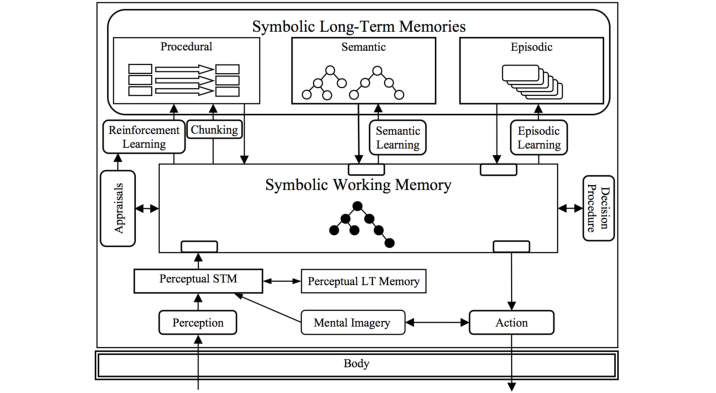
\includegraphics[width=\textwidth]{img/The-Soar-cognitive-architecture.png}
    \caption{The Soar Architecture}
    \label{fig:soar}
\end{figure*}

\begin{itemize}
    \item \textbf{Memory}: multiple memories, mainly divided into \emph{short term working memory} which reflects agent's current circumstances (perceptual inputs, goals, intermediate results), and a \emph{long term memory} which is divided into a
    \begin{enumerate*}[label=(\emph{\roman{*}})]
        \item \emph{procedural memory} containing the production system, a
        \item \emph{semantic memory} which stores facts about the world and the agent itself, and a
        \item \emph{episodic memory} keeping track of agent's past behaviours.
    \end{enumerate*}
    \item \textbf{Grounding}: in embodied context percepts are generated by sensors as agent's inputs, also equipping the Soar agent with actuators allowing physical interactions.
    \item \textbf{Decision Making} accomplished through a decision loop that
    \begin{enumerate*}[label=(\emph{\roman{*}})]
        \item matches preconditions from procedural memory,
        \item checks preconditions against agent's working memory,
        \item through a \emph{propose and evaluate phase} actions ranking and selections is performed for then
        \item choose, produce and execute the action.
    \end{enumerate*}
    \item \textbf{Learning} is supported by the Soar architecture through various forms, where in the most basic ways, facts are written in to semantic memory and experiences in episodic memory. Even behaviours can be modified by rewriting through \ac{RL} or adding new productions to the procedural memory.
\end{itemize}

Cognitive architectures have become less popular over the last few decades
reflecting two main problems: they're \emph{limited to domains} that can be
described with logical predicates, and require many pre-specified rules in order
to function properly.

\subsection{Language Models and Agents}
At its core, a language model is a probabilistic input-output system, where it
learn a distribution $P(w_i|w_{<i})$, where each $w$ is an individual
\emph{token} (word). With the rise of \textbf{Transformer
Based}~\cite{vaswani2023attentionneed} \ac{LLM}s with a large number of
parameters and smart tokenization schemes, along with training on
\emph{internet-scale} text, lead to models useful for many tasks beyond
generating text (e.g. writing code, , etc.). In scenarios where \ac{LLM}s act
in interactive environments, we talk about ''language agents``, i.e. systems
that uses \ac{LLM}s as a core computation unit to reason, plan and act.

\subsubsection{Connections between Language Models and Production Systems}
Formulating the problem of completing a piece of text as a production, allowing
multiple possible continuations, we have $X \rightarrow XY_i$ for some set of
$Y_i$. \ac{LLM}s assign a \emph{probability} to each of these completions.
From this perspective, they defines a probability distribution over \emph{which
productions} to select when presented with input $X$, yielding a distribution
$P(Y_i|X)$ over possible completion.

With this probabilistic approach:
\begin{itemize}
    \item \emph{disadvantages}: opaqueness, uninterpretable and random
        structure makes it challenging to analyze or control their behaviour;
    \item \emph{advantages}: scale and pre-training provide massive advantages
        over traditional production systems.
\end{itemize}

\subsubsection{From Prompt Engineering to Cognitive Language Agents}
Early work on few-shot learning and prompt engineering found that the \ac{LLM}
could be further biased towards high-quality productions by pre-processing the
input string. These manipulation can themselves be seen as productions.
Subsequent works used the \ac{LLM} itself as a pre-processing step, eliciting
targeted reasoning to foreground a particular aspect of the problem or generate
intermediate reasoning steps.

Moreover, when placing the \ac{LLM} in a \textbf{feedback loop} (e.g. Inner
Monologue~\cite{huang2022innermonologueembodiedreasoning} and
ReAct~\cite{yao2023reactsynergizingreasoningacting}) with the external
environment, generate systems that move beyond pre-defined prompt chains: they
first transform multimodal input into text and pass it to the \ac{LLM}, whose
output is then parsed and used to determine an external action.

Later work developed more sophisticated language agents that performs
intermediate reasoning by means of an \ac{LLM} before selecting an action, and
also incorporate learning strategies such as reflecting on episodic memory to
generate new semantic inferences, or modifying their procedural code to
generate new semantic knowledge.

Cognitive architecture has been used to structure production systems'
interactions with agents' internal state and external environment, and the
authors suggest that they can help design \ac{LLM}-based cognitive agents.
